\documentclass{beamer}
\usetheme{Berlin}
\usepackage{color}
\usepackage{natbib}
%\usepackage{multirow}
\usepackage{hyperref}


\setbeamertemplate{itemize subitem}{\tiny\raise1.5pt\hbox{\donotcoloroutermaths$\blacktriangleright$}}

\begin{document}
	\title{Code-based, open-source software for teaching \\ interactive data visualisation}
%	\author{Shan-I Lee}
	\institute{Department of Statistics\\ The University of Auckland}
	
	\date{November 16, 2017}		
	\author{Shan-I Lee, BSc (Hons)\\ Supervisor: Paul Murrell}
	

		\titlepage

	
\section{Introduction}
\label{sec:introduction}
	
	\begin{frame}
		\frametitle{Problem}
		\begin{block}{\citet[p.~25]{Tukey}}<+->
			\textit{Today, software and hardware together provide far more powerful factories than most statisticians realize, factories that many of today's most able young people find exciting and worth learning about} 
		\end{block}
	\begin{itemize}[<+->]
		\item How does interactivity benefit data analysis?
		\item <.-> Which interactive techniques are 'worth learning'? 
		\item <.-> Which code-based, open-source software to use? 
	\end{itemize}
	\end{frame}

	\begin{frame}
		\frametitle{Method}
		\begin{itemize}
			\item Literature review of interactive techniques.
			\begin{itemize}
				\item Interactive data visualisation using \textbf{GGobi} graphical user interface \citep{Cook}
			\end{itemize}
			\item Survey of current code-based, open-source software.
			\item Explore how interactive techniques further insight into data.
			\begin{itemize}
				\item Application to exploratory data analysis (EDA) of the 2016 National Certificate of Educational Achievement (NCEA) results for Auckland schools.
			\end{itemize}
		\end{itemize}
	\end{frame}

\section{Findings}
\label{sec:findings}

	\begin{frame}
		\frametitle{Findings}
		\begin{itemize}
			\item Key interactive techniques that enrich data analysis:
			\begin{itemize}
				\item Linked brushing
				\item Identification
				\item Subset selection
				\item Scaling 
				\item Tours
			\end{itemize}
			\item A focal set of \textbf{R} packages for applying interactive data visualisation: \textbf{plotly}, \textbf{crosstalk} \& \textbf{shiny}.
			\begin{itemize}
				\item Coverage of key interactive techniques
				\item Ease of installation and application
			\end{itemize}
		\item The benefits of interactivity justify the effort of teaching interactive tools.
		\end{itemize}
	\end{frame}

\section{Techniques}
\label{sec:techniques}

	\begin{frame}
		\frametitle{Leveraging static plots}
		\href{https://shanl33.shinyapps.io/presentation_pcp/}{Parallel coordinates plot (PCP)} 
		%\href{files/Demo1_PCP.mp4}{\beamergotobutton{Demo}}
		\href{https://screencast-o-matic.com/watch/cbXlcM2oyE}{\beamergotobutton{Demo}}
		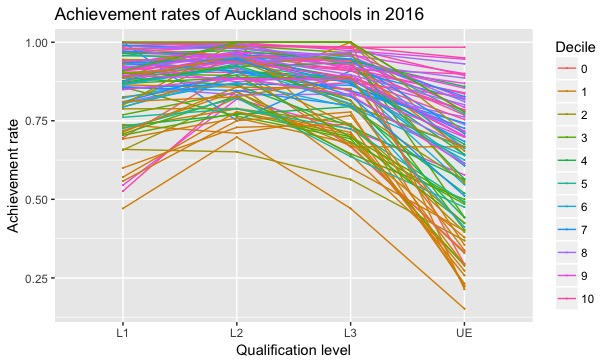
\includegraphics[scale=0.45]{files/pcp.jpeg}
	\end{frame}

	\begin{frame}
		\frametitle{Relating multiple views}
		\href{https://shanl33.shinyapps.io/nceatour/}{Tours} \\
		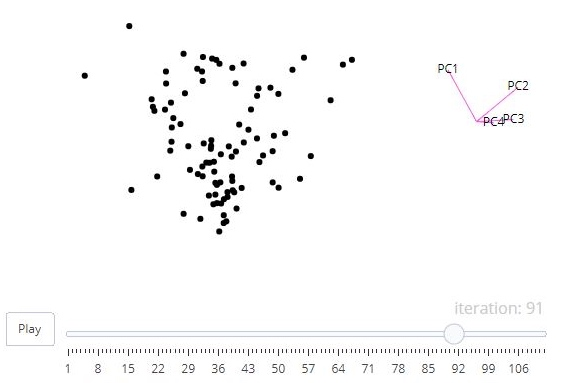
\includegraphics[scale=0.4]{files/tour_hole.jpeg}
	\end{frame}

	\begin{frame}
		\frametitle{Relating multiple views}
			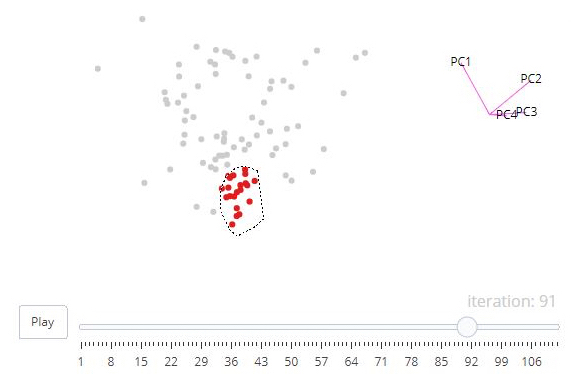
\includegraphics[scale=0.23]{files/tour_brushed2.jpeg}\\
			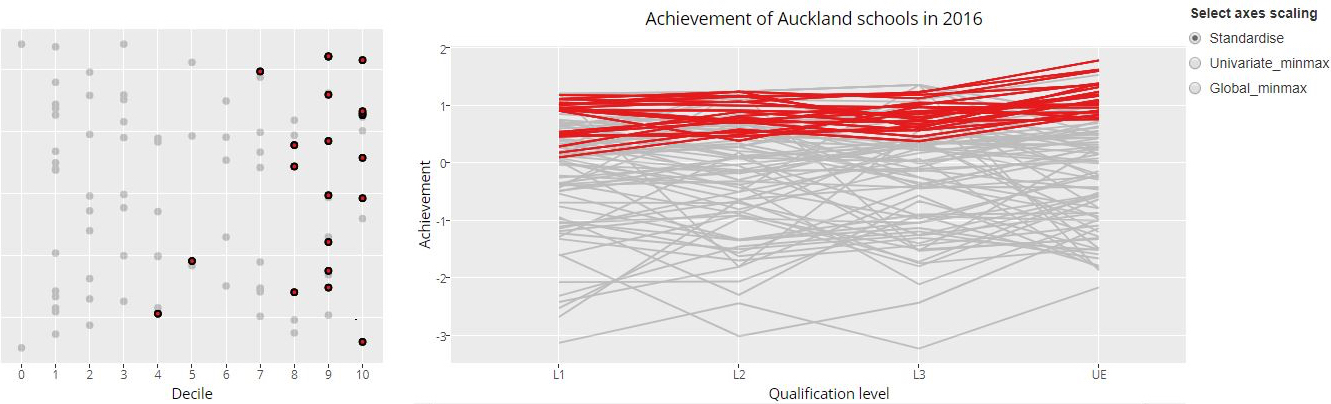
\includegraphics[scale=0.24]{files/link_brush.jpeg}
	\end{frame}

\section{EDA}
\label{sec:EDA}

	\begin{frame}
	\frametitle{Benefits to EDA}
	%Parallel coordinates plot (PCP)
	\begin{itemize}
		\item \textbf{Linked brushing} and \textbf{identification} allowed fast querying of unusual patterns, groups and/or individuals.
		\item \textbf{Subset selection} via filtering views alleviated issues with overplotting and colour schemes.
		\item Interactive \textbf{scaling} revealed different structures.
		\item \textbf{Linked brushing} related multiple views together and helped with interpretation.
		\item \textbf{Tours} allowed multivariate structures to be explored.
		\item Questions were quickly addressed and more questions arose from probing the data with interactive techniques.
	
	\end{itemize}
	\end{frame}

%	\begin{frame}
%		\frametitle{Relating multiple views}
%		\href{run:./multiple.html}{Principal components plot and PCP}
%		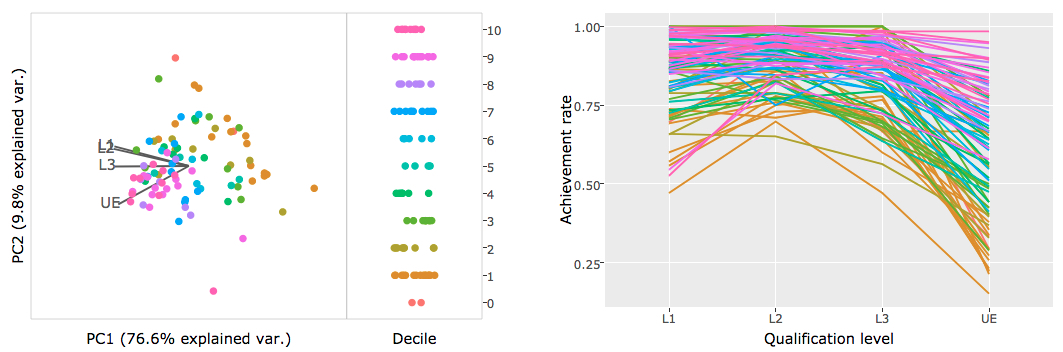
\includegraphics[scale=0.3]{files/PCApcp.jpeg}
%	\end{frame}

%	\begin{frame}
%		\frametitle{Relating multiple views}
%		Principal components plot and PCP
%		\begin{itemize}
%			\item Insights into multivariate data structures gained from individual static plots are extended by \textbf{linked brushing}.
%			\item Applying interactive data visualisation encourages further exploration of the data.
%			\begin{itemize}
%				\item Questions are quickly addressed and more questions arise from probing the data with interactive techniques.
%			\end{itemize}
%			\item Awareness of the strengths and weaknesses of different software allows for efficient application of interactive techniques.
%		\end{itemize}
%	\end{frame}

\section{Software}
\label{sec:software}

\begin{frame}
		\frametitle{A focal set of software}
		Coverage of interactive techniques by \textbf{shiny}, \textbf{plotly} and \textbf{crosstalk}.
		\begin{center}
			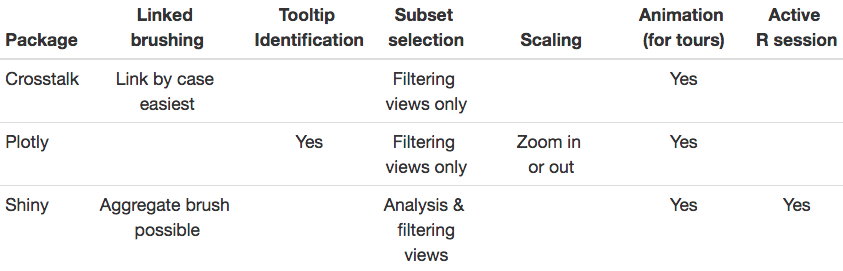
\includegraphics[scale=0.37]{files/table.jpeg}
		\end{center}
\end{frame}

\section{Conclusion}
\label{sec:conclusion}

\begin{frame}
\frametitle{Conclusion}
	\begin{itemize}[<+->]
		\item Interactive techniques benefit data analysis.
		\begin{itemize} 
			\item <.-> Insights beyond static plots
			\item <.-> Utilises and relates multiple views 
			\item <.-> Further exploration of the data
		\end{itemize}
		\item The \textbf{R} packages \textbf{shiny}, \textbf{plotly} and \textbf{crosstalk} enable interactive data visualisation with code-based, open-source software.
		\item The benefits of applying interactive techniques to data analysis warrant teaching interactive data visualisation to future statisticians.
	\end{itemize}
\end{frame}

\begin{frame}[allowframebreaks]{References}
	\bibliographystyle{apalike}
	\bibliography{HonoursProject}
	\nocite{R}
	\nocite{plotly_R}
	\nocite{crosstalk_R}
	\nocite{shiny_R}
\end{frame}

\end{document}